%; whizzy chapter
% -initex iniptex -latex platex -format platex -bibtex jbibtex -fmt fmt
% 以上 whizzytex を使用する場合の設定。


%     Tokyo Debian Meeting resources
%     Copyright (C) 2009 Junichi Uekawa

%     This program is free software; you can redistribute it and/or modify
%     it under the terms of the GNU General Public License as published by
%     the Free Software Foundation; either version 2 of the License, or
%     (at your option) any later version.

%     This program is distributed in the hope that it will be useful,
%     but WITHOUT ANY WARRANTY; without even the implied warranty of
%     MERCHANTABILITY or FITNESS FOR A PARTICULAR PURPOSE.  See the
%     GNU General Public License for more details.

%     You should have received a copy of the GNU General Public License
%     along with this program; if not, write to the Free Software
%     Foundation, Inc., 51 Franklin St, Fifth Floor, Boston, MA  02110-1301 USA

%  preview (shell-command (concat "evince " (replace-regexp-in-string "tex$" "pdf"(buffer-file-name)) "&"))
% 画像ファイルを処理するためにはebbを利用してboundingboxを作成。
%(shell-command "cd image200912; ebb *.png")

%%ここからヘッダ開始。

\documentclass[mingoth,a4paper]{jsarticle}
\usepackage{monthlyreport}
\usepackage{wrapfig}

% 日付を定義する、毎月変わります。
\newcommand{\debmtgyear}{2009}
\newcommand{\debmtgmonth}{12}
\newcommand{\debmtgdate}{12}
\newcommand{\debmtgnumber}{59}

\begin{document}

\begin{titlepage}
\thispagestyle{empty}

% タイトルページ:編集必要な部分は最初のマクロに飛ばすこと

\vspace*{-2cm}
第\debmtgnumber{}回 東京エリア Debian 勉強会資料

\hspace*{-2.4cm}
\includegraphics[width=210mm]{image200801/2008title.eps}\\
\hfill{}\debmtgyear{}年\debmtgmonth{}月\debmtgdate{}日

\end{titlepage}


\dancersection{Introduction}{上川 純一}

\begin{multicols}{2}
 
 
 今月のDebian勉強会へようこそ。これからDebianの世界にあしを踏み入れると
 いう方も、すでにどっぷりとつかっているという方も、月に一回Debianについ
 て語りませんか?

 Debian勉強会の目的は下記です。

 \begin{itemize}
 \item \underline{Debian Developer} (開発者)の育成。
 \item 日本語での「\underline{開発に関する情報}」を整理してまとめ、アップデートする。
 \item \underline{場}の提供。
 \begin{itemize}
  \item 普段ばらばらな場所にいる人々が face-to-face で出会える場を提供
	する。
  \item Debian のためになることを語る場を提供する。
  \item Debianについて語る場を提供する。
 \end{itemize}
 \end{itemize}		

 Debianの勉強会ということで究極的には参加者全員がDebian Packageをがりがり
 と作るスーパーハッカーになった姿を妄想しています。情報の共有・活用を通し
 て Debianの今後の能動的な展開への土台として、「場」としての空間を提供す
 るのが目的です。

 2009年の計画は仮です。

 \begin{enumerate}
  \item 新年の企画 (アンサンブル荻窪開催)
  \item OSC Tokyo
  \item VAIO P インストール記録、
	カーネル読書会 ディストリビューション大集合(小林さん)(東京大学?)
  \item Git Handson (岩松)(あんさんぶる荻窪?)
  \item 家Debianサーバ vs 職場のネットワーク(千代田区都立図書館?\footnote{\url{http://www.library.chiyoda.tokyo.jp/}})
  \item Asterisk (東京大学?)
  \item スペインにて開催
  \item Debconf報告会
  \item OSC Fall?
  \item udev + HAL(岩松さん)
  \item 3D graphics 開発(藤沢さん) 
  \item Debian サーバ+VMware + 各種OS、
	他の仮想化ツール(vserver etc.)、
	忘年会
 \end{enumerate}

 会場候補としては下記があります:

 \begin{itemize}
  \item 大学
  \item 恵比寿SGIホール
  \item Googleオフィス
  \item 公民館(あんさんぶる荻窪等)
  \item 都立会議室(無線LAN)
  \item 健保の施設
 \end{itemize}

\end{multicols}

\newpage

\begin{minipage}[b]{0.2\hsize}
 \definecolor{titleback}{gray}{0.9}
 \colorbox{titleback}{\rotatebox{90}{\fontsize{80}{80} {\gt デビアン勉強会} }}
\end{minipage}
\begin{minipage}[b]{0.8\hsize}
\hrule
\vspace{2mm}
\hrule
\tableofcontents
\vspace{2mm}
\hrule
\end{minipage}

\dancersection{事前課題}{上川 純一}

今回の事前課題は以下です:

\begin{enumerate}
 \item 2009年を振り返って自分は何をしたか
 \item 2009年を振り返ってDebian関連で世間では何が起こったか
\end{enumerate}

この課題に対して提出いただいた内容は以下です。

%; whizzy-master ../debianmeetingresume200912.tex
% $B0J>e$N@_Dj$r$7$F$$$k$?$a!"$3$N%U%!%$%k$G(B M-x whizzytex $B$9$k$H!"(Bwhizzytex$B$,MxMQ$G$-$^$9!#(B

\begin{prework}{$B>e@n=c0l(B}
\preworksection{2009$BG/$r?6$jJV$C$F<+J,$O2?$r$7$?$+(B}

2009$BG/!"H>J,$/$i$$$7$+(BDebian$BJY6/2q$K$O;22C$7$F$^$;$s!#(B

DDTSS $B$r$3$=$3$=$d$C$F$^$7$?$,!"5$$E$$$?$i:#G/$O(BDDTSS$B$N%5!<%P$,$H$^$C$?(B
 $B$j$H$$$m$$$m$H5/$-$?$h$&$G$9!#(B
%$BDI5-$9$k(B

\preworksection{2009$BG/$r?6$jJV$C$F(BDebian$B4XO"$G@$4V$G$O2?$,5/$3$C$?$+(B}

Netwalker $B$,%j%j!<%9$5$l$^$7$?$M!#(B
%$BDI5-$9$k(B

\end{prework}

\begin{prework}{$B5HED=SJe(B}
\preworksection{2009$BG/$r?6$jJV$C$F<+J,$O2?$r$7$?$+(B}
Debian$B4X78$@$H(BDDTSS$B$G%l%S%e!<$rCf?4$K(B180$B7oDxEY$d$C$F$$$?$h$&$G$9!#(B
DDTSS$B$O5Y$s$@$j$d$C$?$j!"$^$C$?$j$d$C$F$$$^$9!#(B
$B%$%Y%s%H4XO"$G$O(B2$B7n$K(BLinux conf.au$B$K9T$C$F!"=)$O(BJLS$B$K%\%i%s%F%#%";22C!"(B
KOF$B$K9T$C$F4X@>(BDebian$B$NJ}$H%-!<%5%$%s$r$7$?$j$7$F$$$^$7$?!#(B
$B$"$H$ONcG/DL$j!)$"$s$I$-$e$a$s$F$C$I$G$S$"$s$N%4!<%9%H%(%G%#%?!<7sGd$j;R$H$7$F!"(B
$BK?=j$GJY6/2q;qNA$r$^$H$a$FK\$K$7$FHRI[$7$F$$$^$9!#(B
\preworksection{2009$BG/$r?6$jJV$C$F(BDebian$B4XO"$G@$4V$G$O2?$,5/$3$C$?$+(B}
$B$d$O$j(BLenny$B%j%j!<%9$,0lHV$G$7$g$&!#(B
$B4pK\E*$K(Bstable$B$r;H$&%A%-%s$J$N$G!"%a%8%c!<%P!<%8%g%s%"%C%W$OBg$-$J(B
$B%K%e!<%9$G$9!#(B
$B:G6a$N(BDebian$B$ODj4|E*$K%j%j!<%9$5$l$k$N$G3F<o%=%U%H$b%P!<%8%g%s$,(B
$B3d$H?7$7$/!"JXMx$K46$8$F$$$^$9!#(B
$B$*$+$2$G;H$$$?$$%=%U%H$N$?$a$K!"(Bsid$BEy$+$i%P%C%/%]!<%H$7$?$j!"(B
$B$=$N$[$+(Btar$B%\!<%k$+$i%S%k%I$9$kI,MWEy$b>/$J$/$J$j!"$^$?$=$N>l9g$N<j4V$b(B
$B@N(B(woddy$B$N:"(B)$B$KHf$Y$F$+$J$j8:$C$F$*$j$"$j$,$?$$$G$9!#(B
\end{prework}

\begin{prework}{$B$^$($@$3$&$X$$(B}
\preworksection{2009$BG/$r?6$jJV$C$F<+J,$O2?$r$7$?$+(B}

$B%h%a$K(B Debian (Sid)$B$r;H$o$;;O$a$?!"(BHack Cafe, Debian JP Project $B$NA*5s4I(B
 $BM}0Q0w!"(BDebian $BJY6/2q$N1?1D$d!"$O$8$a$F$N(B ITP, DebConf9 $B;22C!"$O$8$a$F(B
 $B$N<9I.Ey!"$A$g$3$A$g$3$d$C$F$-$^$7$?$,!"$d$m$&$H;W$C$F$$$?$3$H$O$J$+$J(B
 $B$+$G$-$F$$$J$$$N$,8=>u$G$9!#(B(ITP$B$7$CJ|$7$K$7$F$7$^$C$F$$$k$7!D!#(B)

$BMhG/$O!"$b$&$9$3$7%^%k%A%?%9%/$G!JMWNNNI$/!KF0$1$k$h$&$K$7$?$$!"$H$$$&$+(B
$B$7$J$$$H$$$+$s$J$!$H;W$&G/$N@%$G$7$?!#(B

\preworksection{2009$BG/$r?6$jJV$C$F(BDebian$B4XO"$G@$4V$G$O2?$,5/$3$C$?$+(B}

OpenBlockS 600 $B$,=P$^$7$?$M!#(BOpenBlockS 266 $B$[$ILLGr$_$O$J$$$G$9$,!"%9%Z%C(B
 $B%/$,>e$,$C$F$b>CHqEENO$,Dc$$(B(5W)$B$N$ONI$$$G$9$M!#(B
\end{prework}

\begin{prework}{$B$d$^$M$R$G$-(B}
\preworksection{2009$BG/$r?6$jJV$C$F<+J,$O2?$r$7$?$+(B}
$B0J2<$G4v$D$+$N9`L\$KJ,$1$F?6$jJV$C$F$_$^$9!#(B

\subsubsection{$B%Q%C%1!<%8$N:n@.$H0];}(B}
$B<g$K%U%)%s%H$N%Q%C%1!<%8$K$D$$$FDI2C$r<B;\$7$^$7$?!#0J2<$,DI2C$5$l$?%Q%C%1!<%8$G$9!#(B

\begin{itemize}
 \item ttf-umefont - $B!VG_%U%)%s%H!W$N%Q%C%1!<%8$G$9(B
 \item ttf-umeplus - PCLinuxOS$B$NI8=`%U%)%s%H(B umeplus $B$N%Q%C%1!<%8$G$9!#(B
 \item ttf-ipafont/ttf-ipafont-jisx0208/otf-ipafont - IPA$B%U%)%s%H$G$9!#(B
 \item ttf-monapo - mona$B%U%)%s%H$H(BIPA$B%U%)%s%H$N9g@.%U%)%s%H$G$9(B
 \item ttf-sawarabi-gothic -$B!V$5$o$i$S%4%7%C%/!W%U%)%s%H$G$9!#(B
 \item ttf-misaki - $B!VH~:i%U%)%s%H!W$G$9!#(B
 \item ttf-kanjistrokeorders -$B!V4A;z$N=q$-=g!W%U%)%s%H$G$9!#F|K\8l3X=,<T$K?M5$$G$9!#(B
\end{itemize}

$B$"$H$O(B ITP $B$7$?$^$^:n6H$,;_$^$C$F$$$?$j(B reject $B$5$l$F:FD4@0$,$G$-$F$$$J$$$N$,4v$D$+$"$j$^$9$N$G!"(B
$B$=$l$rJRIU$1$F$$$1$l$P$H;W$$$^$9!#(B

\subsubsection{$BK]Lu:n6H(B}
$B%&%'%V$K$D$$$F$O!"(BDevelopers News $B$N::FI$dK]Lu:n6H!"$=$l$+$i(B po-debconf $B$N99?7$H?75,K]Lu:n6H$r<B;\$7$F$$$^$9!#(B
$B;DG0$J$,$i(B i18n.debian.net $B%5!<%P$,@5>o$K2TF/$7$F$$$J$$$N$G!"(Bpo-debconf $B$N?JD=>u67$O:rG/$HHf$Y$F$I$NDxEY>e$,$C$F$$$k$N$+$OITL@$G$9$,!"8eB`$O$7$F$$$J$$$O$:$G$9!J8=>u$G(B 70\% $B0J>e$O:n6H$7$F$$$k!K!#(B

$B$"$H$O(B upstream $B$G2?$+$G$-$l$P!"$H;W$$!"$3$3?tF|$G$O$"$k$b$N$N(B GNOME $B$NK]Lu99?7:n6H$K<j$r=P$7$F$_$F$$$^$9!#(B
2.30 $B%j%j!<%9$N:"(B (2010/3 $B$+$J!)(B) $B$K92$F$:$K::FI$^$G$G$-$l$PNI$$$G$9$M!#(B

\subsubsection{$B%$%Y%s%H!?9-Js7O$J3hF0(B}
Debian/Ubuntu$B3hF04XO"$G5-;v$r>/$7=q$+$;$F$$$?$@$$$?$j!"BPCL$K;22C$5$;$F$b$i$C$?$j$7$F$$$^$7$?!#(B

\begin{itemize}
 \item Software Design 2009/07 $BFC=8!V=i?4<T$K$d$5$7$/!$%Y%F%i%s$bK~B-!*!V(BDebian GNU/Linux 5.0$B!J(BLenny$B!K$r$*4+$a$9$kM}M3!W(B
 \item Software Design 2009/10 $B!V(BDebian GNU/Linux$B%+%s%U%!%l%s%9!V(BDebconf9$B!W<h:`%l%]!<%H(B Debian$B3+H/<T$,=8$&%9%Z%$%s(B14$BF|4V!W(B
 \item ThinkIT$B!V(BTOMOYO Linux$BE0Dl2rK6!!Bh(B3$B2s!'(BDebian$B$G(BTOMOYO Linux$B$r;H$&!W(B
 \item ascii.jp$B!V9T$C$H$1!*(BUbuntu$BF;>l!W(B
 \item $B%"%9%-!<%a%G%#%"%o!<%/%9!V=54)%"%9%-!<JL:}(B $B$5$/$5$/(BUbuntu!$B!W(B
\end{itemize}

$B$^$?!"%$%Y%s%H$K4v$D$+;22C$7$^$7$?!#:#G/$OBND4$,0-$+$C$?$3$H$b$"$j!":rG/$h$j>/$J$a$G$9(B (KOF$B$H$+9T$1$J$+$C$?!D(B)

\begin{itemize}
 \item Linux Consortium 10 Years Event !!$B!V%*!<%W%s%=!<%9%G%9%/%H%C%W$NL$Mh!W(B(2009/01)
 \item $BBh(B17$B2s%*!<%W%s%=!<%9%F%/%N%m%8!<JY6/2q!w(BGREE Labs$B!J(B2009/04$B!K(B
 \item Ubuntu 9.04 $B%*%U%i%$%s%_!<%F%#%s%0(B (2009/04)
 \item Open Source Conference Tokyo/Fall (2009/11)
\end{itemize}

$B>e5-$NCf$G!"<B<AE*$KH/I=$7$?$N$O(B GREE Labs $B$@$1$G$7$?$N$G!"MhG/$O$b$&>/$7BND4$r@0$($F!"%M%?$r$+$^$;$l$P!"$H;W$$$^$9!#(B


\subsubsection{Debconf9 $B;22C(B}
$B$h$&$d$/(B Debconf $B$K;22C$9$k$3$H$,$G$-$^$7$?!#$,!"$H$j$"$($:9T$C$?$@$1$G=*$o$C$F$k$N$G!"(B
$B$b$&>/$7<B@S$r@Q$`$3$H$H1Q8l$G$N%3%_%e%K%1!<%7%g%s$r2~A1$G$-$l$P$H;W$C$F$$$^$9!#(B

\preworksection{2009$BG/$r?6$jJV$C$F(BDebian$B4XO"$G@$4V$G$O2?$,5/$3$C$?$+(B}
$B$&!<$s!"@$4V$H$$$&$H$=$s$J$K%$%s%Q%/%H$OM?$($i$l$F$$$J$$$+$J!<$H8D?ME*$K$O46$8$F$$$^$9!#(B
\end{prework}

\begin{prework}{$BK\>190E5(B}
\preworksection{2009$BG/$r?6$jJV$C$F<+J,$O2?$r$7$?$+(B}

$B;E;v$,K;$7$/JY6/2q$b7g@J$7$,$A$G$7$?!#(B
$BL@F|$+$i4hD%$k!#(B

\preworksection{2009$BG/$r?6$jJV$C$F(BDebian$B4XO"$G@$4V$G$O2?$,5/$3$C$?$+(B}

SmartQ5$B$,=P$^$7$?!#(B
\end{prework}

\begin{prework}{$B%-%?%O%i(B}
\preworksection{2009$BG/$r?6$jJV$C$F<+J,$O2?$r$7$?$+(B}

$BD>@\(B Debian $B$G$J$/?=$7Lu$J$$$N$G$9$,!&!&!&!#(B
$B$3$N=)!"<B2H$K(B ADSL $B0z$-$^$7$F!"(B Ubuntu $B%$%s%9%H!<%k$7$?%N!<%H(B PC $B$r(B
$BCV$$$F$-$^$7$?!#!!%M%C%H%5!<%U%#%s@lMQ5!$G$9$,!"F@$KJ86g$b$J$/IaDL$K(B
$B;H$C$F$$$k$h$&$G$9!#!!(Bdebian $B7O(B linux $B%f!<%6$r0l?MA}$d$7$?$H$$$&$3$H$G!#(B

\preworksection{2009$BG/$r?6$jJV$C$F(BDebian$B4XO"$G@$4V$G$O2?$,5/$3$C$?$+(B}

$BF17oB??t$+$bCN$l$^$;$s$,!"(B Lenny $B%j%j!<%9$G$9$+$M!#(B
$B@$4V$X$N%$%s%Q%/%H$O!&!&!&!";d$N$^$o$j$G$O$"$^$j$J$+$C$?$h$&$J!)!*(B
\end{prework}

\begin{prework}{$BF|HfLn(B $B7<(B}
\preworksection{2009$BG/$r?6$jJV$C$F<+J,$O2?$r$7$?$+(B}

\begin{itemize}

\item Debian$BJY6/2q$G(BC$B$d(BPerl$B0J30$N8@8l$K$bCmL\$7$F$b$i$*$&$H!"(BOCaml$B$d(BCommon Lisp$B$NI[653hF0$r$7$^$7$?!#(B
\item Debian$BJY6/2q$G(BCommon Lisp$B%M%?$NH/I=$r$7$^$7$?!#(B

\end{itemize}

\preworksection{2009$BG/$r?6$jJV$C$F(BDebian$B4XO"$G@$4V$G$O2?$,5/$3$C$?$+(B}

\begin{itemize}

\item lenny$B%j%j!<%9!#2q<R$N%^%7%s$b%"%C%W%G!<%H$,I,MW$K$J$C$FBgJQK;$7$+$C$?!#(B
\item Debian$BJY6/2q$N1c2q$G$N%h%?OC$b$-$C$+$1$N0l$D$K$J$C$F!"F|K\$G$O=i$N(BOCaml$BFC2=%$%Y%s%H!"(B OCaml Meeting Tokyo 2009$B$G3+:E!#$_$J$5$s$K46<U!#(B

\end{itemize}

\end{prework}

\begin{prework}{$B4d>>(B $B?.MN(B}
\preworksection{2009$BG/$r?6$jJV$C$F<+J,$O2?$r$7$?$+(B}
\begin{itemize}
\item Debian Developer$B$K$J$C$?!#(B\\
Debian Developer$B$K$J$C$?$N$G!"%9%]%s%5!<$r9T$&$h$&$K$7$?!#(B
$B$$$^$^$G$d$C$F$b$i$C$?$3$H$r$d$k$h$&$K?4$,$1$k$h$&$K$7$F$$$k!#(B

\item Debian JP Project Leader $B$K$J$C$?!#(B
$B$J$<$+(B DJPL $B$J$C$F$$$k!#(B

\item Debian SH4 Port $BI|3h(B\\
Debconf9$B$K$$$C$F(B $BB>$N(BPorter$B$H:n6H$,$G$-$?$N$,Bg$-$$!#(B
$B$3$N@.2LJ*$rMxMQ$7$?@=IJ$b=P$?$h$&$G$9!#(B

\item $B;R6!$,@8$^$l$?(B
$B;R6!$,@8$^$l$?$N$G!"@83h$,0lJQ$7$?!#(B

\end{itemize}

\preworksection{2009$BG/$r?6$jJV$C$F(BDebian$B4XO"$G@$4V$G$O2?$,5/$3$C$?$+(B}
\begin{itemize}
\item Lenny $B$,%j%j!<%9$5$l$?(B
\item GPG$B80(B 4096R $B$X$N0\9T(B
\item glibc $B$+$i(B eglibc $B$X$N0\9T(B
\end{itemize}

\end{prework}


\dancersection{最近のDebian関連のミーティング報告}{まえだこうへい}
\subsection{東京エリアDebian勉強会58回目報告}
% (query-replace-regexp "<.*?>" "")
% (query-replace-regexp "^[	 ]\+" "")

東京オリンピック青少年総合センターで開催しました。参加者は、あけどさん、
なかおさん、吉田さん、やまねさん、山本さん、本庄さん、日比野さん、あらき
さん、高橋(emasaka)さん、つじたさん、岩松さん、まえだの12名でした。

Debian での数学ことはじめとして、gnuplot, Octave, Rの入門についての話を
まえだが行いました。gnuplot と R でのプロットのやり方と、R と Octave の
それぞれの拡張パッケージである CRAN, Octave-Forge からの Debian パッケー
ジ化するためのポイントポイントについて議論できたので、参加された方は
gnuplot と Rを自習して使えるようになると同時に、Octave-Forge と CRAN の
拡張パッケージをガンガン Debian パッケージにするべく ITP していることで
しょう。

もう一つのネタとして岩松さんが Debian auto-builder ネットワークについての
話をされました。Debian を支える重要なシステムであるにも関わらず、このシ
ステムを理解している DD も少ないとのことなので、とても意義のあるセッショ
ンでした。特にドキュメント化されていない loop-depends の対応の話には溜飲
を下ろした人が多かったのではないかと思います。今回の話で、auto-builder
に興味を持ったヒトは、ぜひ Debian/SH4のポーティングに参加しましょう。

宴会は、石臼挽きたて蕎麦と酒肴の店 心粋 参宮橋店にて。Rolf さんが宴会か
ら合流され、宴会場でのキーサインパーティが行われました。

\subsection{Adam C Powell IV 迎撃}
\begin{wrapfigure}{r}{18.5zw}
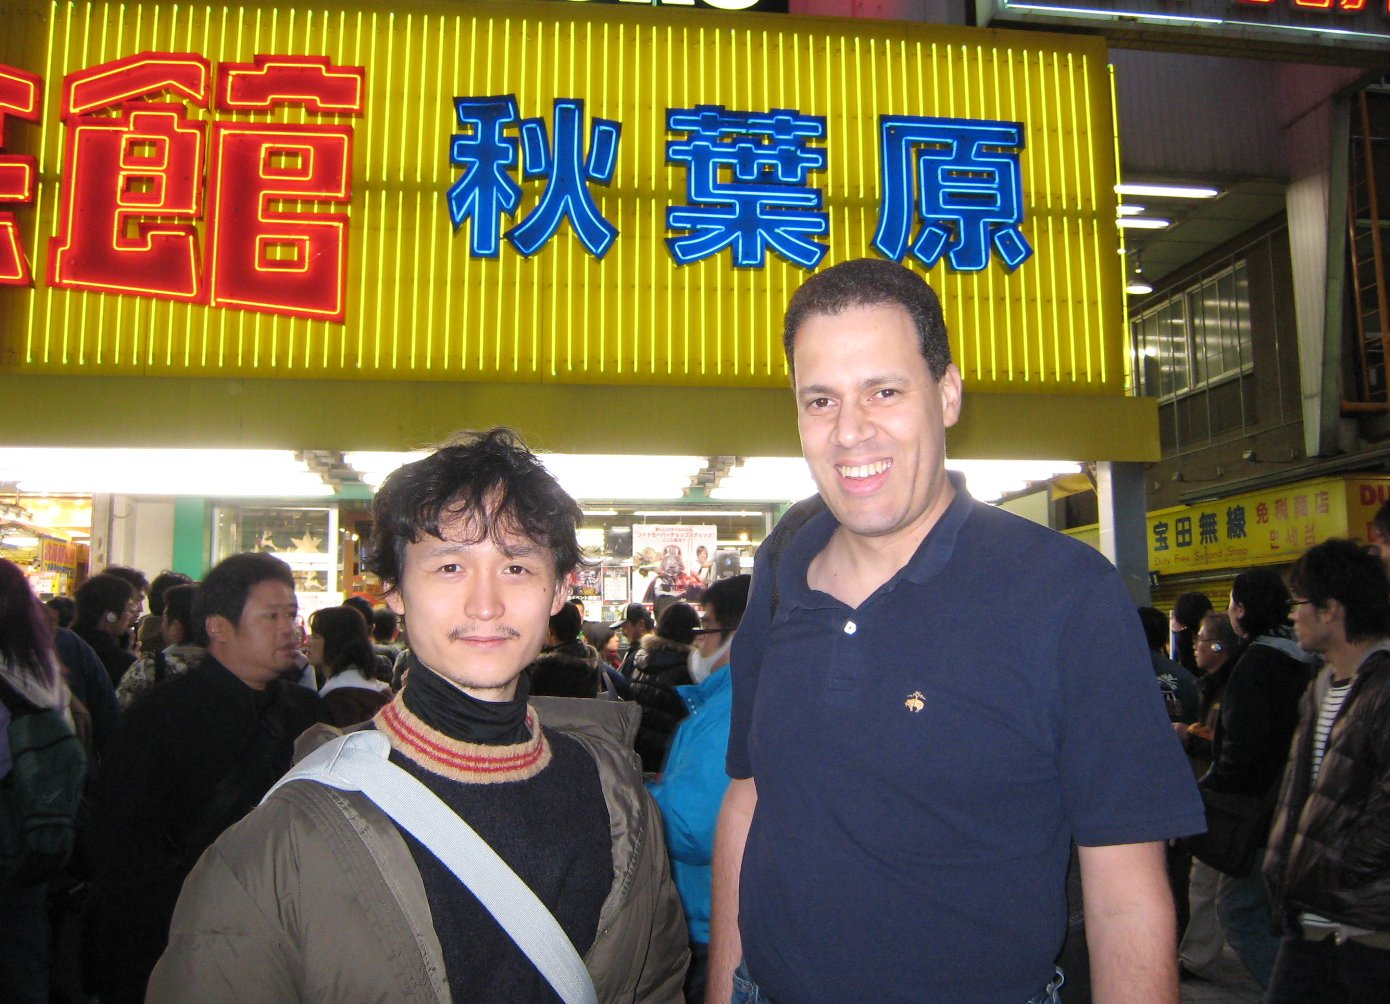
\includegraphics[width=1\hsize]{image200912/acp.jpg}
\end{wrapfigure}

11月29日に来日していた Adam C Powell IV を上川が迎撃しました。
Debian Beowulf Project で昔からやりとりしていた仲です。
秋葉原にいって大喜びしていました。

その直前にDebian Developerの荒木さんとも一緒に飲みに行っていたようです。

\subsection{Dirk Eddelbuettel 迎撃}

11月26日に来日していた Dirk Eddelbuettel を迎撃しました。gtachさん、だい
ごさん、岩松さん、前田さん、Dirk Eddelbuettel 夫妻、上川x2にて宴会。
Debianと金融について熱く語る新宿の夜でした。


% =======================================================================
\dancersection{東京エリアDebian勉強会 2009年度各種イベント開催実績と総括}{上川 純一}
\label{sec:debmtg2009results}
\index{debianjp@Debian JP} 
\index{とうきょうえりあ@東京エリアDebian勉強会}
\index{2009ねん@2009年}

今月で5年目のDebian勉強会が終了しました。
Debian Developerになった人がいたり変化もみられ、私生活の面でも
結婚したメンバーが多数いたり、
転職したメンバーがいたり、当時と所属が変わっていないメンバーのほうがめず
らしくなってきました。

\subsection{Debian勉強会の野望の進捗具合}

今年はDebian勉強会にとって大きなできごとがありました。
当初の目標であったDebian Developerの育成という目標がすこしづつ実現してき
たのです。東京エリアDebian勉強会常連の岩松さん、関西Debian勉強会立ち上げ時
期に尽力した矢吹さんがDebian Developerになりました。苦節5年。おめでとう
ございます。

2009年までは基本的なDebian開発者になるまでの基本的な教養の共有を目的にやっ
てきました。これからは少し方向性を変えて開発に必要な実践的な内容にシフト
していってよいかと考えています。2010年はスポンサー、NMU、BSPの行い方をよ
り実践的に行える方向を模索したいと思います。

\subsection{運営方法}

2009年の勉強会には上川半分くらいしか出席しておらず、
岩松・前田が中心として運営にあたりました。

事前課題は latex のソースコードに対する git format-atch の出力をMLに投稿
するという手順で、宴会君と atnd を補助的に利用しました。
勉強会会場の予約はとりあえず30人くらいが入れる場所を確保しましたが、
宴会会場の予約は人数の確定する開催二日前、でした。

勉強会の会費は500円を維持しています。過去荻窪の「あんさんぶる荻窪」という
公民館を利用していたので、費用計算もそこを基準におこなってきていました。
2009年はいろいろな会場を試しており、公営ではない施設も試しており、会場費
用の高騰にともない赤字決算になった回もあります。公営の施設を利用している
と会場が非常に安かったので印刷費用がまかなえていました。

幹事は昨年までは上川が集中的にしていたので運営についてのノウハウが十分伝
わっていなかった苦労もあったみたいです。

\subsection{基本的な数値}

Debian 勉強会は毎回事前課題事後課題を設定しており、予習復習を必要だとう
たっている勉強会です。
実際にどれくらいの人が出席しているのか、またその人たちがどれくらい事前課
題・事後課題を提出しているのか、確認してみましょう。
\fgref{fig:attendandprepostwork}です。
値は一年の移動平均です。

\begin{figure}[ht]
 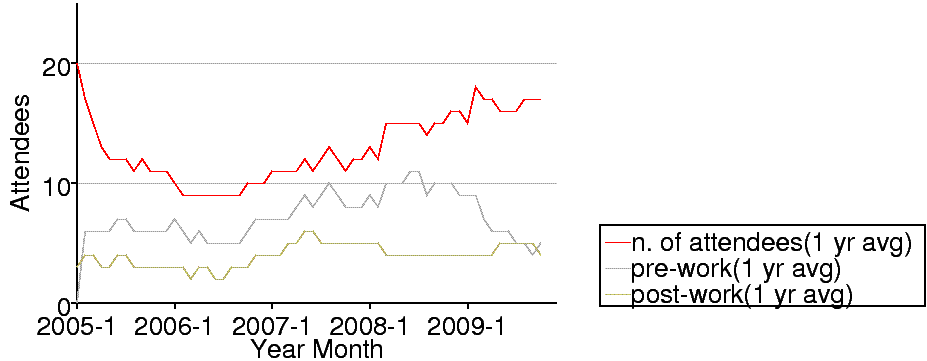
\includegraphics[width=1\hsize]{image200912/memberanalysis/attend.png}
\caption{東京エリアDebian勉強会事前課題・事後課題提出実績(12ヶ月移動平均)}\label{fig:attendandprepostwork}
\end{figure}

毎回の参加者の人数と、その際のトピックを見てみます。今年の場合は、平日の
夜に行ったGPGキーサインパーティーの参加者の多さが目立っています。
 
\begin{table}[ht]
\begin{minipage}{0.5\hsize}
 \caption{東京エリアDebian勉強会参加人数(2005-2006年)}\label{tab:count}
 \begin{center}
  \begin{tabular}{|l|c|p{10em}|}
 \hline
   & 参加人数 & 内容 \\
 \hline
   2005年1月 & 21 & 秘密\\
   2005年2月 & 10 & debhelper 1\\
   2005年3月 & 8 &  (早朝) debhelper 2、social contract\\
   2005年4月 & 6 & debhelper 3\\
   2005年5月 & 8 & DFSG、dpkg-cross、lintian/linda\\
   2005年6月 & 12 & alternatives、d-i\\
   2005年7月 & 12 & toolchain、dpatch\\
   2005年8月 & 7 & Debconf参加報告、ITPからアップロードまで\\
   2005年9月 & 14 & debconf\\
   2005年10月 & 9 & apt-listbugs、バグレポート、debconf翻訳、debbugs\\
   2005年11月 & 8 & DWN翻訳フロー、statoverride\\
   2005年12月 & 8 & 忘年会\\
   2006年1月 & 8 & policy、Debian勉強会でやりたいこと\\
   2006年2月 & 7 & policy、multimedia \\
   2006年3月 & 30 & OSC: debian勉強会、sid \\
   2006年4月 & 15 & policy、\LaTeX{} \\
   2006年5月 & 6 & mexico \\
   2006年6月 & 16 & debconf、cowdancer\\
   2006年7月 & 40 & OSC-Do: MacBook Debian \\
   2006年8月 & 17 & 13執念 \\
   2006年9月 & 12 & 翻訳、Debian-specific、oprofile \\
   2006年10月 & 23 & network、i18n会議、Flash、apt \\
   2006年11月 & 20 & 関西開催: bug、sid、packaging \\
   2006年12月 & 14 & 忘年会 \\
 \hline
  \end{tabular}
 \end{center}
\end{minipage}
\begin{minipage}{0.5\hsize}
 \caption{東京エリアDebian勉強会参加人数(2007-2008年)}\label{tab:count2007}
 \begin{center}
  \begin{tabular}{|l|c|p{10em}|}
 \hline
 & 参加人数 & 内容\\
 \hline
   2007年1月 & 15 & 一年を企画する \\
   2007年2月 & 13 & dbs, dpatch\\ 
   2007年3月 & 80 & OSC仮想化 \\
   2007年4月 & 19 & quilt, darcs, git\\
   2007年5月 & 23 & etch, pbuilder, superh \\   
   2007年6月 & 4 & エジンバラ開催:Debconf7 実況中継 \\
   2007年7月 & 18 & Debconf7 参加報告\\
   2007年8月 & 25 & cdn.debian.or.jp \\   
   2007年9月 & 14 & exim \\   
   2007年10月 & 30 & OSC Tokyo/Fall(CUPS) \\   
   2007年11月 & 19 & live-helper, tomoyo linux kernel patch, server\\
   2007年12月 & 11 & 忘年会\\
   2008年1月 & 23 & 一年を企画する \\
   2008年2月29+3月1日 & 36 & OSC  \\
   2008年3月 & 37 & データだけのパッケージ、ライセンス \\
   2008年4月 & 17 & バイナリパッケージ \\
   2008年5月 & 20 & 複数のバイナリパッケージ \\
   2008年6月 & 10 & debhelper \\
   2008年7月 & 17 & Linux kernel patch / module パッケージ \\
   2008年8月 & 10 & Debconf IRC会議とDebian温泉 \\
   2008年9月 & 17 & po4a, 「Debian メンテナのお仕事」 \\
   2008年10月 & 11? & OSC Tokyo/Fall \\
   2008年11月 & 17 & 「その場で勉強会資料を作成しちゃえ」 Debian を使った \LaTeX{} 原稿作成合宿 \\
   2008年12月 & 12 & 忘年会 \\
 \hline
  \end{tabular}
 \end{center}
\end{minipage}
\end{table}

\begin{table}[t]
\begin{minipage}{0.5\hsize}
 \caption{東京エリアDebian勉強会参加人数(2009年)}\label{tab:count2009}
 \begin{center}
  \begin{tabular}{|l|c|p{10em}|}
 \hline
 & 参加人数 & 内容\\
 \hline
   2009年1月 & 12 & 一年を企画する \\
   2009年2月 & 30 & OSC パッケージハンズオン\\ 
   2009年3月 & 23 & Common Lisp, パッケージ作成 \\
   2009年4月 & 15 & Java Policy, ocaml, 開発ワークフロー\\
   2009年5月 & 13 & MC-MPIパッケージ化、Erlang、Androidアプリ、DDTP \\   
   2009年6月 & 14 & DDTP・DDTSS、bsdstatsパッケージ、Debian kFreeBSD\\
   2009年7月 & ? & スペインにてDebconf 9\\
   2009年8月 & 14 & スペイン Debconf 9 参加報告 \\   
   2009年9月 & 26 & GPGキーサインパーティー \\   
   2009年10月 & ? & OSC Tokyo Fall\\
   2009年11月 & 12 & Octave, R, gnuplot, auto-builder \\
   2009年12月 & ? & 忘年会\\
 \hline
  \end{tabular}
 \end{center}
\end{minipage}
\end{table}


%=================================================
\dancersection{関西 Debian 勉強会\newline2009年度各種イベント開催実績と総括}{倉敷・佐々木・野方}
\index{2009ねん@2009年}
\index{かんさいでびあん@関西Debian勉強会}

\subsection{運営状況}

関西は運営に関わっている人に学生が多いので、いろいろ無理をお願いする場
面も多かったような気がします。

\subsubsection{勉強会全体}

今年度途中(7月)より、運営担当が山下尊也から倉敷・佐々木・野方の三名体制
に交代しました。これは山下の身辺が多忙になり身動きがとれないという理由
からです。幸い、以前より分担に向け運営の見直しを進めていたこともあり、
大きな混乱もなく継続することができました。

年度当初、ライブ中継に若干盛り上がりを見せましたが、その後、うまく継続
できませんでした。問題としてはIPアンリーチャブルな会場をメインにしてい
ることと、中継の実作業を担っていた人が運営側にシフトし、余力を回せなく
なっていることが原因と思われます。

5月には神戸市を中心とした関西地域の新型インフルエンザ流行により、勉強
会を中止する出来事がありました。
社会的な要因により勉強会開催の判断を迫られる状況は初めてでしたが、こう
いう事は二度とあって欲しくないですね。

9月は京都リサーチパークにお邪魔して勉強会初の京都で開催しました。会場を
変えると、いつもとは違う参加者も増えるので、たまに場所を変えるのもよい
のではと思いました。

講師については現状、固定化している中、継続して常連参加者への講師依頼を
するほかに、DMCを取り入れたり、LT発表も可能な参加者自己紹介の常設な
どをおこないました。

LT発表可能な参加者自己紹介は、話題にバリエーションが加わったなど興味深
いこともあった反面、年度後半は関西の勉強会参加者も参加している Open
Street Mapにトピックを持っていかれてしまった感もあり、うまくバランスを
取る必要がありそうです。

また、今年度は佐々木、山下の 2 名が Package Maintainer として
Debian の New queue に新しくパッケージを送り込みました。来年も
この流れを維持できればと思います。

\subsubsection{扱ったテーマ}

勉強会の内容としては、パッケージ開発自体に加えて、Debian の体制にまつわ
る話(gpg や mentors など)や、周辺ツールの利用(bash や reportbug や gdb
など)をとりあげました。
来年度のテーマについては、年末年始に相談をする予定をしています。

翻訳関連では、東京での流れに乗りDDTSSのハンズオン実習をしましたが、予想
外に反応がありました。もともと需要があったのか、実習したことで身近になっ
たのか、はよくわかりませんが…。

\subsubsection{イベント関連}
例年通り、夏のオープンソースカンファレンスKansai@Kyoto(OSC)と、秋の関
西オープンフォーラム(KOF)に出展しました。

セッションでは、OSCでは大浦さんによるDebian GNU/kFreeBSDについて、KOFで
は矢吹さんにDDになるまでの軌跡をお話してもらいました。
矢吹さんは、関西Debian勉強会立ち上げの立役者なので、できれば勉強会にも
来て欲しいところですが、最近は、なかなかご多忙で難しいとのことです。

また、四国ではじまったオープンフォース勉強会 \footnote{
\url{http://openforce.project2108.com/}}と、岡山でのオープンセミナー
@岡山 \footnote{\url{http://openseminar.okaya.ma/}} に、野方が参加して
Debian Liveやノウハウの紹介などを行いました。

\subsection{開催実績}

関西Debian勉強会の出席状況を確認してみましょう。
グラフで見ると\fgref{fig:kansaipeoplechart}になります。
表で見ると\tbref{tab:count2009kansai} です。

\begin{figure}[h]
 \begin{center}
  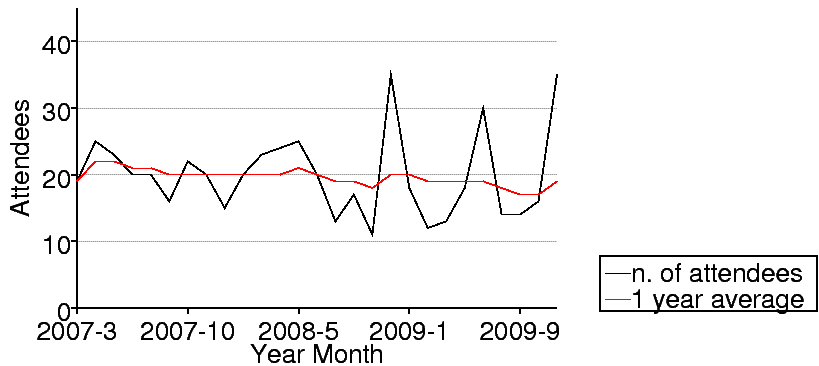
\includegraphics[width=1\hsize]{image200912/kansai.png}
 \end{center}
\caption{関西の参加人数推移}
\label{fig:kansaipeoplechart}
\end{figure}

\begin{table}
\begin{minipage}{0.5\hsize}
 \caption{関西Debian勉強会参加人数(2007年)}\label{tab:count2007kansai}
 \begin{center}
  \begin{tabular}{|l|c|p{10em}|}
 \hline
 & 参加人数 & 内容 \\
 \hline
2007年3月 & 19 & 開催にあたり \\
2007年4月 & 25 & goodbye、youtube、プロジェクトトラッカー\\
2007年6月 & 23 & 社会契約、テーマ、debian/rules、bugreport\\
2007年7月 & 20前後 & OSC-Kansai \\
2007年8月 & 20 & Inkscape、patch、dpatch\\
2007年9月 & 16 & ライブラリ、翻訳、debtorrent\\
2007年10月 & 22& 日本語入力、SPAMフィルタ\\
2007年11月 & 20前後 & KOF \\   
2007年12月 & 15& 忘年会、iPod touch\\   
 \hline
  \end{tabular}
 \end{center}
\end{minipage}
\begin{minipage}{0.5\hsize}
 \caption{関西Debian勉強会参加人数(2008年)}\label{tab:count2008kansai}
 \begin{center}
  \begin{tabular}{|l|c|p{10em}|}
 \hline
 & 参加人数 & 内容 \\
 \hline
2008年2月 & 20 & PC Cluster, GIS, \TeX \\
2008年3月 & 23 & bug report, developer corner, GPG \\
2008年4月 & 24 & coLinux, Debian GNU/kFreeBSD, sid \\
2008年5月 & 25  & ipv6, emacs, ustream.tv\\
2008年6月 & 20  & pbuilder, hotplug, ssl\\
2008年8月 & 13  & coLinux \\
2008年9月 & 17  & debian mentors, ubiquity, DFSG\\
2008年10月 & 11  & cdbs,cdn.debian.or.jp \\
2008年11月 & 35  & KOF \\
2008年12月 & ?  & TeX資料作成ハンズオン\\
 \hline
  \end{tabular}
 \end{center}
\end{minipage}
\begin{minipage}{0.5\hsize}
 \caption{関西Debian勉強会参加人数(2009年)}\label{tab:count2009kansai}
 \begin{center}
  \begin{tabular}{|l|c|p{10em}|}
 \hline
 & 参加人数 & 内容 \\
 \hline
2009年1月 & 18 & DMCK, LT \\
2009年3月 & 12 & Git \\
2009年4月 & 13 & Installing sid, Mancoosi, keysign \\
2009年6月 & 18 & Debian Live, bash\\
2009年7月 & 30? & OSC2009Kansai \\
2009年8月 & 14 & DDTSS, lintian \\
2009年9月 & 14 & reportbug, debian mentors\\
2009年10月 & 16 & gdb, packaging \\
2009年11月 & 35 & KOF2009 \\
2009年12月 & ?? & GPS program, OpenStreetMap \\
 \hline
  \end{tabular}
 \end{center}
\end{minipage}
\end{table}

%=================================================
\dancersection{2009年を振り返ってみる}{上川 純一}
%=================================================
\index{2009ねん@2009年}

\subsection{最近のトレンドと今後の推移}

最近どんなことが
あって、これからどういうことがあるでしょうか。
みんなで予想してみましょう。

{\footnotesize
\begin{tabular}[t]{|p{8em}|p{8em}|p{12em}|p{8em}|p{8em}|}
\hline
2007 &2008 &2009 & 2010 & 2011 \\
\hline
%2007
VT・AMD-V(仮想化技術)が普及(ML115!)、

玄箱(ARM)、
OpenBlocks(PPC?)、
iPhone登場、 
HSDPA 月額5000円くらいに、
google mobile、

VISTAリリース、 
Leopardリリース、 

GPL3.0、
メモリ2Gがコモディティーに、
SparcT2がオープン、 
ニコニコ動画、
& 
%2008
python 3.0
ruby 1.9

wine 1.0, wine64 登場

RoR 2.0 登場で普及に

4コア・64bit のCPUがデスクトップに普及、
Core2Quad 値下げ。

ニコニコ動画1000万ユーザ突破、
初音ミクブームに

地デジ関連のPC製品の普及

勉強会の普及(楽天とか)

公衆無線LAN (wireless gate)

携帯電話の売上が落ちる、
iPhone, Android 登場、
emobile 100円PC抱きあわせ
(eeePC, Dell mini9)
Zaurus販売終了。

Chumby 発売。

サーバの仮想化 ESXi・シンクライアント

MacBook Air 発売、
無線 802.11n が実機に

SystemZ10 発表

世界経済の崩壊(IT投資緊縮財政、職を失う人が増加)

FreeBSD 7 (malloc, ZFS ?)

Debian次世代育成計画始動

Debian Maintainer 制度始動

セキュリティー関連(OpenSSL 事件、DNS事件)

クラウド関連が流行?

Nintendo DSi

&
%2009
政権交代,スパコン事業仕分け,円高

Windows7,Snow Leopard発売

Netwalker発売

MacBookからIEEE1394が消えた。

メモリがDDR3に移行中,メモリ高騰

マジコン販売取り締まり

ラブプラス,OSSを使ったエロゲー登場(OpenCV),AR,セカイカメラ

JLSでLinus来て大騒ぎ

DD,2世誕生

デジタルサイネージ

Google Voice,Wave,Chrome,Chrome OS,Go,日本語入力,徒歩ナビ

CouchDB

Twitter,*なうブーム

Eye-Fi,Kindle2,DS LL,PSP-GO,POKEN

Cell終了のお知らせ

tile window manager boom ?

Lenny リリース

Debian 結婚ブーム

デスクトップ、4コア、8GB

ノートパソコン、2コア、4GB

Linux が標準インストールのPC。(Dell)

SSD の値段と容量がこなれる(まあまあ)
HDDがなくなる?高くなる?(ならず)

SSD特化したFSが出てきた

ipv6 使えるようになってる(来年)

DL禁止法? torrent に逆風?

&
%2010
Debian OAuthサービス開始のお知らせ

SolidICE使ったDebian VDIサービス開始のお知らせ

Chrome OS,Android統合のお知らせ

Willcom終了のお知らせ

Netbook,クラウド,Amebaなう終了のお知らせ

Debian Cloudリリースのお知らせ

10GbE,SSD普及

新iPhoneリリース

自民復活

SIMロックフリー延期のお知らせ

新Android端末(日本以外)

次世代用FS:btrfs,NILFS

Lenny and Halfリリース

Squeezeリリース遅延,kFreeBSD,SH4 オフィシャルアーキテクチャに

ToyStory3リリース

消費税上昇に伴う繁忙期

クラウドにより、単純なホスティング業者がつづかない?
一部は自社でもつようになる?

USB 3.0 搭載、wireless USB vs Bluetooth ?

組み込みCPUはAtomに統一?Armは残ってる?

ruby 2.0 リリース?Perl6リリース?

&
%2011
Windowsドライバシグニチャチェックがなくなる

IEEE1394終了のお知らせ

LTEが徐々に普及

地デジ延期のお知らせ

Debian 11 日本開催

Googleに統合(オフィスソフト、グループウェア、メール、ファイルサー
		 バ止めようぜ運動)

Scalaのエンタープライズ利用

Windows11リリース

C/Sを意識せずにアプリ開発できる環境(コンパイラが自動判断)

\\

\hline
\end{tabular}

}

\clearpage

%=================================================
\dancersection{qemubuilder 2009年アップデート}{上川純一}
%=================================================
\label{sec:qemubuilder-update2009}
\index{かそうか@仮想化} 
\index{ARM} 
\index{qemu}
\index{qemubuilder}

\subsection{qemubuilderの基本コンセプト}

qemubuilder はDebianパッケージをビルドするためのツールです。debootstrapの
クロスブートストラップ機能を利用してベースイメージを作成した後、qemu を利
用して各アーキテクチャ用の仮想マシンを実行し、その中でパッケージをビルド
します。ネイティブビルドと変わらない使用感でパッケージのビルドができるの
で面倒なクロスビルドの設定が必要ありません。特にDebianパッケージはbuildd
でネイティブビルドされ、クロスビルドされない前提なので、builddでビルドで
きるようなパッケージの作成・デバッグに便利です。

\subsection{qemubuilderの使い方}

利用したいアーキテクチャ向けのカーネルと設定ファイルを用意します。
手元の設定では次のような設定になっています。
\begin{commandline}
KERNEL_IMAGE=vmlinuz-2.6.24-1-versatile-armel
ARCH=armel
BASEPATH=/home/dancer/tmp/base-armel.qemu
INITRD=
\end{commandline}

イメージをまず作成します。これで、BASEPATHに指定したファイル名にqemuの
RAWディスクイメージが作成されます。

\begin{commandline}
# qemubuilder --configfile arm.config --create 
\end{commandline}

ディスクイメージをアップデートします。

\begin{commandline}
# qemubuilder --configfile arm.config --update
\end{commandline}

パッケージをビルドするのには dsc ファイルを指定します。

\begin{commandline}
# qemubuilder --configfile arm.config --build xxx.dsc
\end{commandline}

\subsection{qemubuilderの課題}

カーネルと設定ファイルの取得が今一番面倒なところです。Debianの標準のカー
ネルと initrd でできた時期もあったのですが、現在そういうようにはなってい
ません。

アーキテクチャの組み合わせがあまりにも多いため、動く組み合わせを同定する
ことや、デバッグが困難です。スクリプトで自動化すること、またテストの自動
化が必要ではないかと考えています。

また、qemu の-appendコマンドでカーネルにブートパラメータを指定できること
を装丁していますが、実際にはそれができないアーキテクチャ(ppcなど)があり、
そのままでは動きません。\footnote{いまでもそうかはわかりません}

最近はkFreeBSDアーキテクチャなども登場してきていますが、このままの設計で
はそこまで手が回らなさそうです。

\subsection{qemubuilderの今後の進め方}

どうしましょうね。

%=================================================
\dancersection{lxc コンテナを使ってみる }{まえだこうへい}
\label{sec:lxc}
\index{かそうか@仮想化} 
\index{Linux Kernel Container}
\index{Containers}
\index{lxc}

Debian 勉強会に参加されている面々は、そろそろ Xen や KVM 以外に何かない
のか、新たなネタを求めている向きが多いかと思います。そこで、最近、Linux
Kernel に新たにマージされた機能を使って実現している、lxc という仮想化技
術について紹介します。

\subsection{はじめに}
\subsubsection{lxc の概要}
lxc\footnote{\url{http://lxc.sourceforge.net/}} は、正式名称を Linux
Containers と言い、コンテナ自体が稼働するためのカーネルの機能と、コンテ
ナを管理するためのとユーザツールから構成されます。lxc で使用している
Kernel の機能(Control Group, 以下 Cgroup と省略)は、
kernel 2.6.29 で完全にマージされ、カーネルにパッチを当
ててビルドする必要がなくなってなっています。kernel 2.6.29 より前のカーネ
ルでは、kernel 2.6.27 以降であればパッチを当てれば使うことが
できます。

lxc は GPL2 ライセンスで公開されていて、開発およびメンテナンスは、Daniel
Lezcano 氏が実質一人で行っています。

Debian では、Squeeze/Sid からパッケージ化されており、一つ前の最新版
\footnote{2009年11月27日現在、0.6.3。}がパッケージとなっています。

\subsubsection{他のコンテナ型仮想化技術との比較}

コンテナ型の仮想化技術というと有名なのは、Solaris Containers や FreeBSD
jailがありますが、Linux では Linux-VServer, OpenVZ\footnote{Parallels
Virtuozzo ContainersのOSS版。}などがあります。いずれも既に使ったことがあ
る方が多いのではないのでしょうか。

lxc で提供されるサービスは、大きく分類してシステムコンテナと、アプリケーションコンテナの2
つがあります。前者は、いわゆるOSまるごとの仮想化です。init から起動して、仮想OS
の空間を提供します。後者は、chroot によるアプリケーションの分離に近いで
す。単一アプリケーションを分離するだけなので、とても軽くシンプル
なのが特徴です。

lxc は現状、一人で開発・メンテナンスされており、今後プロジェクト
がどうなるのか先行き見えないところではあります。現在、メーリングリストを見
ている限りでは開発は続いているようです。

\subsection{導入してみる}
\subsubsection{ソースコードを取得する}
ユーザスペースのツールのソースコードは、SourceForge にあります。
ソースコードは git で管理されており、最新版は git リポジトリから取得できます。

\begin{commandline}
$ git clone git://lxc.git.sourceforge.net/gitroot/lxc/lxc
\end{commandline}

Debian では前述のとおり、Squeeze/Sid でパッケージになっている
\footnote{\url{http://packages.debian.org/search?keywords=lxc&searchon=names&exact=1&suite=all&section=all}}
ため、最新版である必要がなければ、ソースコードは特に必要ありません。

\subsubsection{カーネルオプションを有効にする}
lxc の機能をフルに活用するには以下のカーネルオプションが有効になっている
必要があります。

\begin{commandline}
* General
  * Control Group support
    -> namespace cgroup subsystem
    -> cpuset support
    -> Group CPU scheduler
    -> control group freeze subsystem
    -> Basis for grouping tasks (Control Groups)
    -> Simple CPU accounting
    -> Resource counters
    -> Memory resource controllers for Control Groups
    -> Namespace support
    -> UTS namespace
    -> IPC namespace
    -> User namespace
    -> Pid namespace
  * Network support
    -> Networking options
      -> Network namespace support
\end{commandline}

これらが有効になっているかを確認するには、lxcのソースツリーに含まれている、
src/lxc/lxc-checkconfig.in というシェルスクリプトを実行すれば、現在起動
中のカーネルでどのカーネルオプションが無効になっているかをチェックできま
す。

また、Debian パッケージでは、/usr/bin/lxc-checkconfig としてインストール
されています。Squeeze/Sid で Debian のカーネルパッケージ\footnote{2009年
11月27日現在、linux-image-2.6.30-2-amd64}を使っている環境で確認すると以
下の結果になります。Cgroup memory controller のみが無効になっているよう
です。

\begin{commandline}
$ lxc-checkconfig 
Kernel config /proc/config.gz not found, looking in other places...
Found kernel config file /boot/config-2.6.30-2-amd64
--- Namespaces ---
Namespaces: enabled
Utsname namespace: enabled
Ipc namespace: enabled
Pid namespace: enabled
User namespace: enabled
Network namespace: enabled
Multiple /dev/pts instances: enabled

--- Control groups ---
Cgroup: enabled
Cgroup namespace: enabled
Cgroup device: enabled
Cgroup sched: enabled
Cgroup cpu account: enabled
Cgroup memory controller: disabled
Cgroup cpuset: enabled

--- Misc ---
Veth pair device: enabled
Macvlan: enabled
File capabilities: enabled
\end{commandline}

\subsubsection{Debian でのインストール}

ここから先は、Squeeze/Sid でパッケージを使うことを前提として話を進めます
が、このままでは、cgroup でのメモリ管理は無効になっていますので、カーネ
ルオプション \verb!CONFIG_CGROUP_MEM_RES_CTLR! を有効にしてリビルドしてください。
それ以外で実際に Debian で lxc を使うために必要なパッケージは何かというと
lxc だけです。

\begin{commandline}
$ sudo apt-get install lxc
\end{commandline}

これでアプリケーションコンテナを試すことはできます。README にも載ってい
る手順ですが、次のコマンドを実行すると、即席のコンテナを起動できます。

\begin{commandline}
$ uname -a
Linux silicon 2.6.32 #1 SMP Sun Dec 6 02:30:30 JST 2009 x86_64 GNU/Linu
$ sudo lxc-execute -n hoge -f ./lxc-macvlan.conf /bin/bash
# uname -a
Linux alpha 2.6.32 #1 SMP Sun Dec 6 02:30:30 JST 2009 x86_64 GNU/Linux
\end{commandline}

他のコンソールからコンテナが起動しているか確認してみます。

\begin{commandline}
$ sudo lxc-info -n hoge
'hoge' is RUNNING
$ lxc-ps -n hoge 
CONTAINER    PID TTY          TIME CMD
            4747 pts/3    00:00:00 bash
            5692 pts/3    00:00:00 lxc-ps
            5693 pts/3    00:00:00 ps
\end{commandline}

ちゃんと確認できましたね。今回は、これで以上です、と言いたいところですが、
この環境はコンテナを起動させただけでしかなく、はっきり言って役に立ちませ
ん。bash を sudo で起動しているだけで、ホスト OS のファイルシステムにも
アクセスできてしまいます。

コンテナだけを起動させて満足、はい、終了とするのであれば良いかもしれませ
んが、実際に lxc を活用しようと考えているなら次に挙げる他のパッケージを
インストールし、さらにコンテナ用のクローズ環境を作る必要があります。

\begin{itemize}
 \item iproute : コンテナのネットワーク設定を行うため。
 \item debootstrap : コンテナのイメージを作成するため。
\end{itemize}

今回は、クローズな Debian 環境を簡単に作るための方法を紹介します。
\footnote{厳密に言うと、コンテナからホスト OS で稼働しているプロセスや、
カーネルメッセージが見えてしまうのでクローズにはまだなっているとは言えま
せんが、まだ開発中でもあるのでそのうち改善されるでしょう。}

\subsubsection{ネットワークの設定}
\subsubsubsection{\textbf{ブリッジの設定}}

必要なパッケージをインストールしたら、まずはブリッジの設定を行う必要があります。
/etc/network/interfaces で直接ブリッジの設定をすれば良いと思いますが。シェ
ルスクリプトを用意して、それをpost-up で実行させれば良いでしょう。

\begin{commandline}
#!/bin/sh

brctl addbr br0                             <- ブリッジデバイスの追加
brctl setfd br0 0                           <- ブリッジデバイス br0 の設定
ifconfig br0 192.168.0.1 promisc up
brctl addif br0 eth0
ifconfig eth0 0.0.0.0 up
route add -net default gw 192.168.0.254 br0 <- ホスト OS のゲートウェイ
\end{commandline}

interfaces は以下のように設定します。
\begin{commandline}
$ cat /etc/network/interfaces 
# This file describes the network interfaces available on your system
# and how to activate them. For more information, see interfaces(5).

# The loopback network interface
auto lo
iface lo inet loopback

# The primary network interface
auto eth0
allow-hotplug eth0
iface eth0 inet static
	address 192.168.0.101
	netmask 255.255.255.0
	broadcast 192.168.0.255
	pre-up  /etc/init.d/iptables start
	post-up /etc/network/if-up.d/brctl.sh
\end{commandline}

以上のあと、ブリッジの設定がきちんとされているか確認してみると、以下のよ
うになります。
\begin{commandline}
$ /usr/sbin/brctl show
bridge name	bridge id		STP enabled	interfaces
br0		8000.00wwwwyyyyxxno		eth0
							veth0_14820
							veth0_15932
							veth0_17164
\end{commandline}
ちなみに``veth0\_''の後ろの数字は、コンテナで起動した init プロセスのプロセスID
です。


\subsubsubsection{\textbf{IP フォワードと NAT の設定}}

ホスト OS とコンテナ、コンテナとホスト OS の外部のネットワーク、コンテナ
間での通信は、上記の設定だけでなく、IP フォワードや NAT の設定をする必要
があります。例えば、コンテナ起動後、ホスト OS から ssh でログインするの
にも、IP フォワードが必要となります。

\begin{commandline}
$ sudo bash -c ``echo 1 > /proc/sys/net/ipv4/ip_forward''
\end{commandline}

IP フォワードを設定するととで、ホスト OS の外部のネットワークへの通信や、
コンテナ同士の通信も行えるようにはなります。\footnote{同じブロードキャス
トドメインの場合。}

一方、ホスト OS の外部ネットワークからはこのままではアクセスできません。
アクセスを許可するには、ホスト OS でポートフォワーディングや、宛先 NATな
どを行う必要があります。ポートフォワーディングを行うのであれば、以下のよ
うなルールを設定します。

\begin{commandline}
iptables -t nat -A PREROUTING -d 192.168.0.1 -p tcp --dport 80 -i br0 -j DNAT --to 192.168.0.101
iptables -t nat -A PREROUTING -d 192.168.0.1 -p tcp --dport 5984 -i br0 -j DNAT --to 192.168.0.102
\end{commandline}

ここでの設定は、デフォルトポリシーが全て ACCEPTであることを前提にしてい
ますが、実際には当然 DROP にすると思いますので、FORWARD のルールなども定
義する必要があります。Netfilter のルールとIPフォワーディングの許可はスク
リプトにして、/etc/network/interface で pre-up として設定しておくと良い
でしょう。

なお、FORWARD チェインのデフォルトポリシーが ACCEPT である場合は問題あり
ませんが、DROP や REJECT に設定してある場合は、コンテナ同士での通信はで
きません。FORWARD チェインでの ACCEPT ルールが必要になります。

\subsubsection{システムコンテナの作成}
\label{sec:make_container}

では、システムコンテナのイメージを作成してみます。lxc のパッケージに含まれる、
/usr/share/doc/lxc/examples/lxc-debian.gz を使って、Debian のシステムコ
ンテナを作成します。

まず、このファイルをホームディレクトリなどで伸張します。
\begin{commandline}
$ zcat /usr/share/doc/lxc/examples/lxc-debian.gz > ~/lxc-debian
\end{commandline}

次に、cgroup ファイルシステムをマウントします。/etc/fstab に下記一行を追
記します。マウントポイントは任意の場所で構いません。

\begin{commandline}
cgroup  /var/local/cgroup  cgroup  defaults  0  0
\end{commandline}

追記したら、マウントポイントのディレクトリを作成し、マウントします。

\begin{commandline}
$ sudo mkdir /var/local/cgroup
$ sudo mount cgroup
\end{commandline}

それでは、先ほどの lxc-debian スクリプトを使ってコンテナイメージを作成し
ます。このスクリプトでは debootstrap を使ってイメージが作成されますが、
ディストリビューションは lenny になっています。前述した通り本環境は
Squeeze/Sid ですので、コンテナも Squeeze/Sid の方が良ければ、コンテナイ
メージを作成する前に予めスクリプトを書き換えておく必要があります。
また、パッケージも、デフォルトで apache2 がインストールされたり、一方、
sudo や vi, dig コマンドが無かったりするので、そのままインストールすると
不便であったりするので、予めインストールするパッケージの指定を変更してお
く必要があります。lxc-debian スクリプト内の debootstrap コマンドの
\verb/--include/オプションでパッケージの指定は変更できます。
また、sshd の設定や、ネットワークの設定も予め設定しておくと便利です。以
下、変更済みファイルとの diff の結果を掲載しておきます。

\begin{commandline}
$ diff -u  a/lxc-debian b/lxc-debian 
--- a/lxc-debian	2009-11-30 21:22:59.000000000 +0900
+++ b/lxc-debian	2009-10-30 17:58:20.000000000 +0900
@@ -8,8 +8,8 @@
 MNTFILE=
 TMPMNTFILE=
 UTSNAME=
-IPV4="172.20.0.21"
-GATEWAY="172.20.0.1"
+IPV4="192.168.0.101"
+GATEWAY="192.168.0.1"
 MTU="1500"
 
 # These paths are within the container so do not need to obey configure prefixes
@@ -99,14 +99,14 @@
 SyslogFacility AUTH
 LogLevel INFO
 LoginGraceTime 120
-PermitRootLogin yes
+PermitRootLogin no
 StrictModes yes
 RSAAuthentication yes
 PubkeyAuthentication yes
 IgnoreRhosts yes
 RhostsRSAAuthentication no
 HostbasedAuthentication no
-PermitEmptyPasswords yes
+PermitEmptyPasswords no
 ChallengeResponseAuthentication no
 EOF
 }
@@ -259,8 +259,8 @@
 	        # download a mini debian into a cache
 		echo "Downloading debian minimal ..."
 		debootstrap --verbose --variant=minbase --arch=$ARCH \
-		    --include ifupdown,locales,libui-dialog-perl,dialog,apache2,netbase,net-tools,iproute,openssh-server \
-		    lenny $CACHE/partial-$ARCH http://ftp.debian.org/debian
+		    --include ifupdown,locales,libui-dialog-perl,dialog,sudo,vim-tiny,dnsutils,netbase,net-tools,iproute,openssh-server \
+		    sid $CACHE/partial-$ARCH http://cdn.debian.or.jp/debian
 		
 		RESULT=$?
 		if [ "$RESULT" != "0" ]; then
\end{commandline}

それでは、コンテナを作成します。コンテナを作成する場所は任意の場所にでき
ます。通常、lxc-debian スクリプトを実行を実行したディレクトリの下に
debianディレクトリを自動的に作成し、その下にコンテナイメージである
rootfs が作成されます。配置したいディレクトリが無ければ作成し、そのディ
レクトリへ移動し、\texttt{sudo lxc-debian create}を実行します。

\begin{commandline}
$ sudo mkdir /var/cache/lxc
$ cd /var/cache/lxc
$ sudo bash /home/kohei/lxc-debian create
What is the name for the container ? [debian] hoge                 <- コンテナの名前
What hostname do you wish for this container ? [hoge]              <- コンテナのホスト名
What IP address do you wish for this container ? [192.168.0.101]   <- コンテナの IPアドレス
What is the gateway IP address ? [192.168.0.1]                     <- コンテナから見たデフォルトゲートウェイのアドレス
What is the MTU size ? [1500]
Specify the location of the rootfs [./rootfs.hoge]
Specify the location for an extra fstab file [(none)]
(snip)
Choose your architecture
1) amd64
2) i386
#? 1                                                               <- Core 2 Duo のマシンなのでアーキテクチャは amd64 を選択。
Architecture amd64 selected
Checking cache download ...Found.
Copying rootfs ...Done.
(snip)
update-rc.d: using dependency based boot sequencing
Done.

You can run your container with the 'lxc-start -n hoge'
\end{commandline}

これで、/var/cache/lxc/debian/rootfs.hoge という名前でコンテナイメージの
ディレクトリが作成され、ここに、debootstrap による Debian イメージのコピー
が作成されます。初めて \texttt{lxc-debian create} を実行すると、
debootstrap でダウンロードされるキャッシュイメージが、
/var/cache/lxc/debian/rootfs-architecture として作成されます。\footnote{今回は
amd64 を選択しているので、/var/cache/lxc/debian/rootfs-amd64 となります。}

コンテナ自体のメタ情報は、/var/lib/lxc ディレクトリのコンテナ名のディレ
クトリ以下にあります。ツリー表示すると以下のようになっています。

\begin{commandline}
$ tree hoge/
couchdb/
|-- cgroup
|-- config
|-- fstab
|-- init
|-- network
|   `-- veth0
|       |-- ifindex
|       |-- link
|       |-- mtu
|       |-- name
|       `-- up
|-- nsgroup -> /var/local/cgroup/hoge
|-- pts
|-- rootfs
|   `-- rootfs -> /var/cache/lxc/debian/rootfs.hoge
|-- state
|-- tty
`-- utsname

5 directories, 13 files
\end{commandline}

\subsubsection{システムコンテナの起動}

システムコンテナの起動の前に、やることがあります。コンテナイメージに、ロ
グイン可能なユーザアカウントを作成することと、/etc/hosts を書き換えるこ
とです。前者は、コンテナ作成後にそのまま起動させたのでは、ログインするこ
とができません。ホストOS 側と同じユーザアカウントで問題なければ、
/var/cache/lxc/debian/rootfs.hoge/etc/ディレクトリの下の、passwd,
shadow, group をホストのそれで上書きしておくと良いでしょう\footnote{今後
作成するコンテナ全てに共通して言えることなので、キャッシュイメージである、
/var/cache/lxc/debian/rootfs-amd64/etc/ディレクトリ以下を上書きしておい
た方が良いかもしれません。}。後者はコンテナ自身の名前解決の設定が目的で
す。現状では、コンテナの/etc/hosts は、一律、

\begin{commandline}
127.0.0.1	localhost
127.0.1.1	ホストOSのホスト名
\end{commandline}

となっており、上記の2行目が、/etc/hostname と異なるため、ユーザアカウン
トを作っても、ログイン時に名前解決で時間が掛かってしまいます。
ですので、予め、ホストOSのホスト名になっている部分をコンテナのホスト名に書き換えておく必要
があるわけです。\footnote{これは、lxc-debian スクリプト自体でコンテナの
ホスト名を書き換えるようにしておけば済む話だと思うんですけどね。}

上記の設定を終えたら、システムコンテナを起動します。
システムコンテナの起動は、\texttt{lxc-start} コマンドを使います。一つの
環境で複数のコンテナを起動できるので、コンテナ名の指定が必ず必要です。コ
ンテナ名の指定には、オプション\texttt{-n} を使います。

\begin{commandline}
$ sudo lxc-start -n hoge
\end{commandline}

このまま起動させると、現在のシェルでそのままコンテナのコンソールが表示さ
れます。ログインするにはそのままコンソールログインすれば良いでしょう。
バックグラウンドで起動させるには、\texttt{-d} オプションをつけます。

\begin{commandline}
$ sudo lxc-start -n hoge -d
\end{commandline}

KVM や Xen などのようにカーネルから起動させる訳ではなく、init プロセスか
ら起動させるので、起動完了までに要する時間はわずかです。

\subsection{lxc の仕組みを見てみる}
\subsubsection{コンテナのライフサイクル}

Linux コンテナのライフサイクルは他の仮想化技術と大きく異なるところはなく、
次の図の様になります。

\includegraphics[width=0.8\hsize]{image200912/lxc/lxc-lifecycle.eps}

この図での状態を遷移させるためのコマンド、つまりコンテナを管理するための
コマンドは以下の通りです。

{\footnotesize
\begin{tabular}[t]{|p{8em}|p{6em}|p{16em}|p{18em}|}
\hline
status &コマンド &実行後の状態 &備考 \\
\hline
\hline
コンテナの起動 &lxc-start &STARTING, RUNNING &システムコンテナ \\
&lxc-execute & &アプリケーションコンテナ\\
\hline
コンテナの一時停止 &lxc-freeze &FROZEN & \\
\hline
コンテナの再開 &lxc-unfreeze &RUNNING & \\
\hline
コンテナの停止 &lxc-stop &STOPPING, STOPPED & \\
\hline
コンテナの再起動 &lxc-restart &STOPPING, STOPPED & \\
& &STARTING, RUNNING & \\
\hline
コンテナの作成 &lxc-create &STOPPED &lxc-debian は内部でlxc-create を実
	     行。 \\
& & &lxc-fedora, lxc-sshdなども同様。 \\
\hline
コンテナの破棄 &lxc-destroy & & \\
\hline
\end{tabular}}

\subsubsection{リソースを制御する}

lxc では、コンテナのリソースを制御するために、cgroup というカーネルの機
能を使っています。cgroup とは、Control group の略です。
Linux Kernel は通常プロセス単位でのリソース制御を行っていました。
cgroup を使うと、同じ cgroup に所属しているプロセス間でのリソースの共有がで
きます。lxc では、\texttt{lxc-cgroup} コマンドを用い、
コンテナのリソースの設定を表示したり、値をセットすることができます。

\subsubsubsection{設定を変更する。}
cgroup の変数を表示する場合は、``\texttt{lxc-cgroup -n コンテナ名 変数
名}''で、変数の値を変更するには、``\texttt{sudo lxc-cgroup -n コンテナ名
変数名 設定する値}''とします。

例えば、CPU リソースの割り当てには、cpu.shares というパラメータを用いま
すが、あるコンテナに割り当てられている比率を算出するには、\texttt{任意の
コンテナの cpu.shares / 各コンテナの cpu.share の総和}を計算する必要があ
ります。具体的には、現在の各コンテナの cpu リソースの割り当て設定を確認
すると、

\begin{commandline}
$ lxc-ls
couchdb  git  hoge  octave  w3m  web
$ for i in `lxc-ls`; do echo -ne $i"\t"; lxc-cgroup -n $i cpu.shares; done
couchdb	2048
git	1024
hoge	1024
octave	1024
w3m	1024
web	1024
\end{commandline}

総和は7168で、各コンテナは、couchdb は約28.6\%、他のコンテナは約14.3\%ご
との比率で CPU リソースをシェアするということ分かります。

\subsubsubsection{コンテナ全体のリソースは?}
上記の通り、\texttt{lxc-cgroup} コマンドは、コンテナを明示的に指定する必要
があるので、cgroup 管理下全体での使用率などを把握するには不便です。
cgroup で制御されるリソースは\ref{sec:make_container}節でマウントした、
cgroup ファイルシステムからアクセスすることもできます。今回はマウントポ
イントを/var/local/cgroup にしているのでこのディレクトリの下を見てみると
以下の様になっています。\footnote{lxc-cgroup コマンド自体は、各コンテナ
の値を/var/lib/lxc/コンテナ名/nsgroup/以下から取得しますが、これは、
/var/local/cgroup/コンテナ名 へのsymlinkになっています。}

\begin{commandline}
$ cd /var/local/cgroup
$ ls -F
couchdb/               cpuset.memory_pressure           git/
cpu.shares             cpuset.memory_pressure_enabled   hoge/
cpuacct.stat           cpuset.memory_spread_page        net_cls.classid
cpuacct.usage          cpuset.memory_spread_slab        notify_on_release
cpuacct.usage_percpu   cpuset.mems                      octave/
cpuset.cpu_exclusive   cpuset.sched_load_balance        release_agent
cpuset.cpus            cpuset.sched_relax_domain_level  tasks
cpuset.mem_exclusive   devices.allow                    w3m/
cpuset.mem_hardwall    devices.deny                     web/
cpuset.memory_migrate  devices.list
\end{commandline}

/var/local/cgroup ディレクトリ以下にある、``xxx.yyyy''の形式をとっている
のが、cgroupで管理するリソース項目で、このディレクトリ直下はシステム全体
のリソースです。一方、hoge/などのディレクトリがありますが、これは各コン
テナに割り当てられているリソース項目です。ですので、このディレクトリを使っ
て、lxc 全体と各コンテナのリソースの管理を行うことができます。

\subsection{まとめ}

Linux Kernel の標準機能だけを使ったコンテナである、Linux Containers につ
いて説明しました。まだまだ機能的には不十分なところもあり、開発体制も不安
なところはありますが、特別なカーネルパッチを適用せずに試せる点では非常に
気軽に使えるのではないかと思います。

また、lxc は libvirt のサポート対象にもなっています。本資料を作成前に
libvirt で扱えるか検証してみたところ、定義ファイルを作るところまではでき
たものの、virsh でコネクトするとうまくリソースにアクセスできないといった
問題もありますが、やることが多いのでハックするには良いネタになるのではな
いでしょうか。

\subsection{参考文献}

\begin{itemize}
\item LXC\\
      \url{http://lxc.sourceforge.net/lxc.html}

\item LXC: Linux コンテナツール ; IBM developer Works Japan\\
      \url{http://www.ibm.com/developerworks/jp/linux/library/l-lxc-containers/}\footnote{
      今年の2月の記事ですが内容が若干古く、現在存在しないコマンドもある
      ので要注意。}
\item Cgroup And Memory Resource Controller\\
      \url{http://www.linux-foundation.jp/uploads/seminar20081119/CgroupMemcgMaster.pdf}
\end{itemize}

%\printindex

%\cleartooddpage

\vspace*{15cm}
\hrule
\vspace{2mm}

\includegraphics[width=2cm]{image200502/openlogo-nd.eps}
\noindent \Large \bf Debian 勉強会資料\\ \\
\noindent \normalfont \debmtgyear{}年\debmtgmonth{}月\debmtgdate{}日 \hspace{5mm}  初版第1刷発行\\
\noindent \normalfont 東京エリア Debian 勉強会 (編集・印刷・発行)\\
\hrule

\end{document}
